% Preamble
\documentclass[11pt]{article}
\usepackage[letterpaper]{geometry}
\usepackage{cite}
\usepackage{url}
\usepackage{fancyhdr}
% Packages
\usepackage{amsmath}
\usepackage{graphicx}
\usepackage[english]{babel}
\usepackage{lipsum}
\usepackage{wrapfig}
\usepackage[font=small,labelfont=bf]{caption}
\usepackage{xcolor}
\fancypagestyle{firstpage}
{
\fancyhead[L]{}
\fancyhead[R]{Zach Arnold \linebreak CS 7641 \linebreak Assignment 4}
\setlength{\headheight}{52pt}
}
\graphicspath{./}
\newcommand{\problemone}{Small Grid World}
\newcommand{\problemtwo}{Mountain Car}
% Document
\begin{document}
    \thispagestyle{firstpage}


    \section{Introduction}\label{sec:introduction}
    The purpose of this paper is to explore Markov Decision Processes.
    Specifically, analyzing algorithms for solving MDPs in two different problem domains.
    Those domains will have differing characteristics such as state domain, size, and action types in those domains.
    I will attempt to compare the results from three different algorithms, Value Iteration, Policy Iteration, and Q-Learning.


    \section{Problem Descriptions}
    In this section I will talk about the different problems I will be analyzing and why they are interesting.

    \subsection{\problemone}
    This problem is fairly classic in reinforcement learning algorithm analysis.
    The domain of this problem is a 10 x 10 matrix of squares representing a grid which is a subset of the world.
    (See figure~\ref{Fig:Small Grid World} for an example grid world.)
    There are up to 100 unique states in this world and 4 actions that can be taken in any state.
    If we suppose that the grid world were a map with the upward direction being North and the remaining three directions,
    then moving in one of these four directions represent the set of possible actions.
    Associated with each action there are a few parameters I configured:
    \begin{itemize}
        \item Success rate which controls some stochastic actions into the agents actions in the domain. An action taken by the agent will succeed with probability equal to the success rate $\in [0,1]$ and do some other random action otherwise.
        \item Goal reward which controls the reward value of the goal state
        \item Move reward which controls the value for selecting any action and moving to another square on the grid
    \end{itemize}
    Outside of standard walls that bound the outside edge of the grid world I have the option of turning some of the grid
    squares into "walls" themselves in that they cannot be moved into.
    This reduces the total number of states, but can actually make traversing the map harder due to the fact that direct
    routes may not exist.
    I have done this in my grid world problem to exercise the ability of an algorithm (given discount factor) to consider
    other potential paths to the goal state.

    \subsubsection{Why is this problem interesting?}
    This problem is interesting because it exercises many of the core functionalities of the learning and planning algorithms that I am employing.
    Due to its low number of states and actions, as well as its relative simplicity, this problem is compelling in that we should be able to
    quickly derive insights from and still be able to compare to a more complex one.
    Since there is also an element of randomness in the actions taken by an agent, this problem is still reasonably complex
    and requires some form of exploration before directly arriving at an optimal value/policy/Q.
    The introduction of non-traversable squares should exercise the algorithms ability to consider other possible paths
    (even those moving in a direction further from the goal.)

    \subsection{\problemtwo}
    The mountain car problem is also an interesting single agent reinforcement learning MDP problem.
    The problem uses a cosine curve to model a valley and two peaks and the agent needs to find its way via actions to the higher of the two (or the top of the mountain.)
    From the description in the documentation:
    \begin{quote}
        "In this domain you can change the parameters for min/max position and velocity, the scale of the cosine curve on which the car travels, the force of gravity, acceleration, and the amount of time that elapses between simulation/decision steps."\cite{Burlap20}
    \end{quote}
    The actions that an agent can take in this domain are:
    \begin{itemize}
        \item Move Backwards
        \item Move Forwards
        \item Do Nothing
    \end{itemize}

    \subsubsection{Why is this problem interesting?}
    This problem Is interesting given that it has a large number of potential states.
    By large, I mean that it has an infinite number of states given that it is a continuous domain modeled by the cosine curve.
    In order to overcome the requirement by value iteration and policy iteration in BURLAP to be able to determine all
    states that are reachable I will be sampling 5000 states from a uniform distribution positions along this curve.
    Whereas in the grid world there was some stochastic randomness to the transition function between states, the agent
    in this world will have different external forces to overcome, namely the force of gravity and the lack of friction
    whereby an agent could perform no actions and still experience a transition (othwerwise known as momentum.)
    Given all these it will be interesting to see the results of the algorithms on this problem.


    \section{Algorithms}
    In this section we will talk about the algorithms I will be using to analyze these problems as well as the parameters
    that I will vary in search of an optimal solution to these problems.

    \subsection{Parameter Exploration}\label{subsec:parameter-exploration}
    In this subsection I will describe the various parameters that I will be using to tune the solution to the problems.
    Many of these are standard parameters and while I did not perform an exhaustive grid search for each best parameter,
    randomized selection optimizing for performance in terms of iterations and wall-clock time as well as total average
    reward was the strategy I employed to arrive at the values described in the analysis section.
    \begin{itemize}
        \item $\gamma$ which is the discount factor where $\gamma \in [0,1]$ and manages the explore/exploit dilemma in RL where high values favor long-term rewards, and low values optimize for greedier short-term rewards
        \item $\delta$ which controls the threshold that if Policy Iteration, Value Iteration, or Q-Learning improve by less than this value, then the algorithm terminates
        \item Initial Q Value initialized optimitically in my case of 0.3
        \item $\alpha$ which controls the learning rate of the respective algorithms
        \item Number of Trials, which dictates the number of times to re-run a learning session with a particular algorithm, the average reward of which is taken as the final result
    \end{itemize}
    Unless explicitly mentioned all algorithms search in an $\epsilon$-greedy fashion, where $\epsilon = 0.1$

    \subsection{Value Iteration}
    For both problems I used the BURLAP implementation of value iteration to derive the optimal reward values for each state
    according to the Bellman update rule.
    Even though Value Iteration is guaranteed to converge, in order to keep my experiments from taking forever, I leveraged
    from the params above to terminate the updates after a threshold or maxiumum iterations occurs.

    \subsection{Policy Iteration}
    For both problems I used the BURLAP implementation for Policy iteration passing in from the above section the $\delta$,
    and max iterations to control the termination provided that we never improve less than $\delta$ in a Learning episode.

    \subsection{Q-Learning}
    Much like the previous two sections, I leveraged the BURLAP implementation of Q-Learning using the params from above
    which apply to Q-Learning and optimized them for each problem.


    \section{Analysis}
    In the section I will compare the performance of the algorithms on the various problems.
    For the purposes of this paper whenever a "result" was achieved or I declare an algorithm has "converged," that means
    that either the maximum number of iterations was reached and the result remains, or (more likely) that each algorithm
    during its update step increased its value, policy, or Q by less than parameter $\delta$.
    Experiments were performed to determine the appropriate $\delta$ for each problem, but were kept the same for each
    algorithm running against a problem for comparative ease.

    \subsection{\problemone}
    For problem one the results that I gathered are the average of 1,000 trials using the same grid world and parameters.
    After tuning the various parameters from the subsection on parameter definition, I determined that the following were optimal
    values for each algorithm: $\gamma = 0.999, \delta = 0.0001, \alpha = 0.2, Q = 0.5$ as described above each algorithm
    searched in an $\epsilon$-greedy fashion where $\epsilon = 0.1$.
    Table~\ref{tab:\problemone~Results} contains the results of each algorithm on the \problemone.
    The Algorithm which converts the fastest in terms of wall clock time was value iteration by a very small margin.
    All of the algorithms performed roughly similar in terms of wall clock time.
    This is largely expected due to the fact that the world is small and the results fairly direct to compute.
    Interestingly Q learning performed for worse in terms of average number of actions to reach a desired goal state.
    Looking at the policy determined in Figure~\ref{Fig:Small Grid World} from the small grid world even though I placed
    a large number of blocking squares in the way between the agent and the goal, the policy remained remarkably consistent across runs.
    In fact comparing reward per trial between policy ration and valuation yielded very similar graphs as seen by figures~\ref{Fig:Policy Iteration~\problemone},~\ref{Fig:Value Iteration~\problemone}.
    However the value iteration method seem to have a more consistent reward per trial closer to the best possible reward which was 3.0.
    Despite research shown by Kaelbling et al, Policy Iteration should have outperformed Value Iteration given that we had
    a very high discount factor $\gamma = 0.99$.\cite{Kaelbling1996}
    All three algorithms converge to the best and correct answer from my understanding given that they all have the same
    best reward, and the same best number of steps to complete.
    Introducing Q-Learning into the mix shows that while it took longer in terms of iterations and actions,
    it still converged to the same result.
    Without knowing transition probabilities or rewards Q-Learning was remarkably able to arrive at this in only 1.5x
    slower in terms of wall clock time than value or policy iteration.
    Looking at figures~\ref{Fig:Q-Learning DD~\problemone} and~\ref{Fig:Q-Learning~\problemone}, we see that in the
    beginning of the training that Q learning has many more steps than either policy or value iteration.
    However after about episode number 120 the average number of steps begins to settle into the range that value and
    policy iteration have suggesting that Q-Learning has nearly successfully determined the rewards on states at that point
    during training.
    Average award for Q learning appears to be quite spiky suggesting that even into trial number 1000 there was still
    a large amount of variance in terms of the best path through the grid world from the starting stay to the goal state.
    \begin{table}
        \centering
        \begin{tabular}{|c| c | c | c |}
            \hline
            & Policy Iteration & Value Iteration & Q-Learning \\
            \hline
            \hline
            Average Number of Actions & 28               & 28              & 102        \\
            \hline
            Average Reward            & -4.18049         & -4.07429        & -11.45929  \\
            \hline
            Best Number of Actions    & 21               & 21              & 21         \\
            \hline
            Best Reward               & -3.00000         & -3.00000        & -3.00000   \\
            \hline
            Average Processing Time   & 0.217(s)         & 0.214(s)        & 0.355(s)   \\
            \hline
        \end{tabular}
        \caption{\label{tab:\problemone~Results}\problemone~Results}
    \end{table}
    \begin{figure}
        \begin{minipage}{0.5\textwidth}
            \centering
            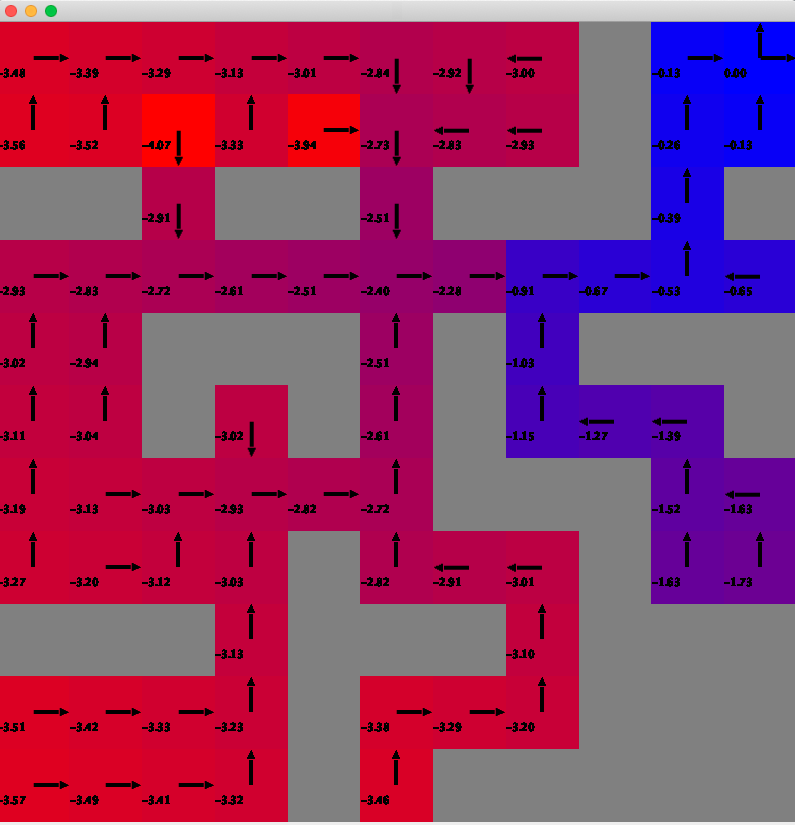
\includegraphics[width=1\linewidth]{smallgridworld.png}
            \caption{Small Grid World}\label{Fig:Small Grid World}
        \end{minipage}
        \begin{minipage}{0.5\textwidth}
            \centering
            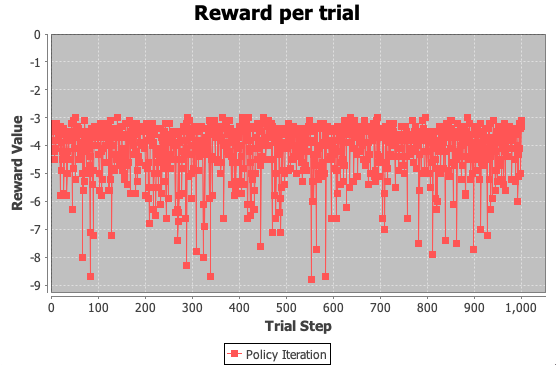
\includegraphics[width=0.99\linewidth]{policyiterationreward.png}
            \caption{Policy Iteration~\problemone}\label{Fig:Policy Iteration~\problemone}
        \end{minipage}
    \end{figure}

    \begin{figure}
        \begin{minipage}{0.5\textwidth}
            \centering
            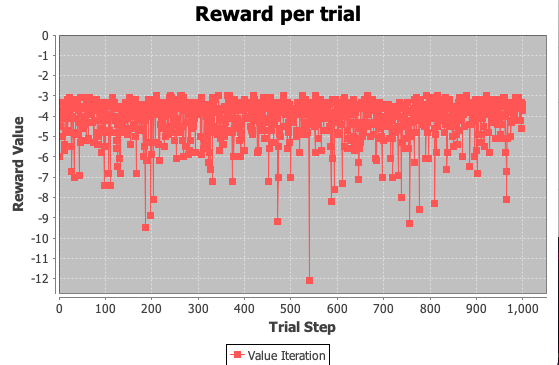
\includegraphics[width=1\linewidth]{valueiterationreward.png}
            \caption{Value Iteration~\problemone}\label{Fig:Value Iteration~\problemone}
        \end{minipage}
        \begin{minipage}{0.5\textwidth}
            \centering
            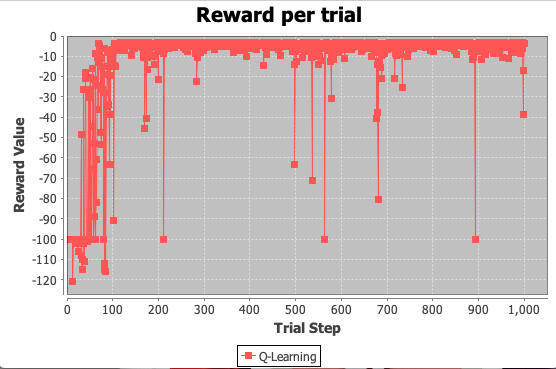
\includegraphics[width=1\linewidth]{qlearningreward.png}
            \caption{Q-Learning~\problemone}\label{Fig:Q-Learning~\problemone}
        \end{minipage}
    \end{figure}
    \begin{figure}
        \begin{minipage}{1\textwidth}
            \centering
            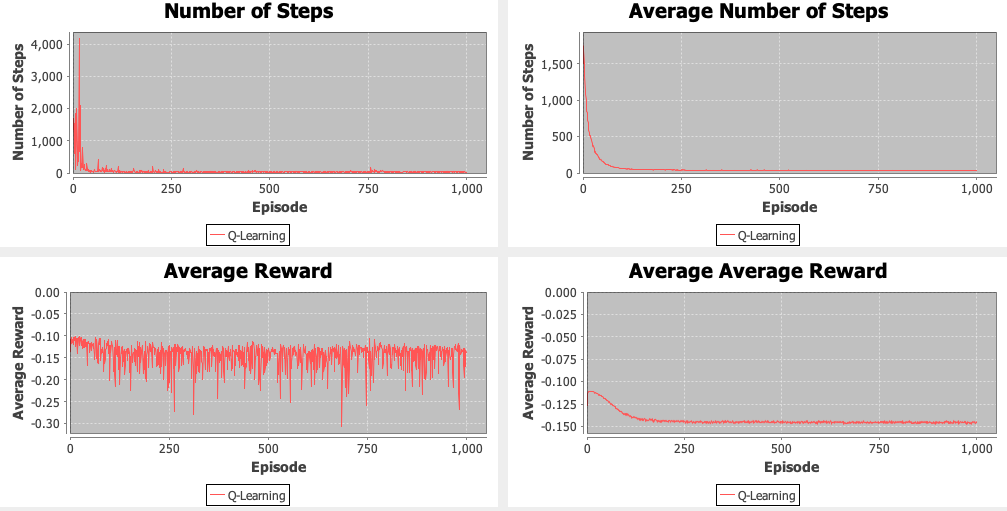
\includegraphics[width=1\linewidth]{qlearningdeepdive.png}
            \caption{Q Learning Analysis~\problemone}\label{Fig:Q-Learning DD~\problemone}
        \end{minipage}
    \end{figure}

    \subsection{\problemtwo}
    In the section I will analyze the results of the three algorithms versus the \problemtwo Problem.
    In my estimation this was a far more interesting test of the various methods to determine the best reward/policy.
    The reason for this is because the state space exists on a continuous domain and not a discreet one.
    See figure~\ref{Fig:Mountain Car} as an example visualization of the statespace and agent.
    Note that the black line is the cosine curve representing the "mountain," and the red block is the "car" that the agent
    is manipulating through the actions described earlier in this paper attempting to determine the sequence of actions
    necessary to use the physics of the environment to get to the top of the curve on the right (the goal state.)
    Because there are essentially an infinite number of states that can be generated in an environment or observed, then
    other methods would need to be used in order to properly enumerate and explore the environment to determine an optimal
    reward or policy.
    To this end, I have simplified this for the sake of completing in a non-infinite amount of time my analysis.
    From the mountain car environment I have sampled 5000 individual state observations and collected them as a set of
    $<s,a,r,s'>$ vectors.
    Table~\ref{tab:\problemtwo~Results} shows the results of each of the algorithms in the environment.
    \begin{table}
        \centering
        \begin{tabular}{|c| c | c | c |}
            \hline
            & Policy Iteration & Value Iteration & Q-Learning \\
            \hline
            \hline
            Average Number of Actions & 164              & 37530           & 47624      \\
            \hline
            Average Reward            & 100              & 100             & 100        \\
            \hline
            Best Number of Actions    & 164              & 1683            & 18646      \\
            \hline
            Best Reward               & 100              & 100             & 100        \\
            \hline
            Average Processing Time   & 20503.0(s)       & 118.1(s)        & 285.9(s)   \\
            \hline
        \end{tabular}
        \caption{\label{tab:\problemtwo~Results}\problemtwo~Results}
    \end{table}

    \begin{figure}
        \begin{minipage}{0.5\textwidth}
            \centering
            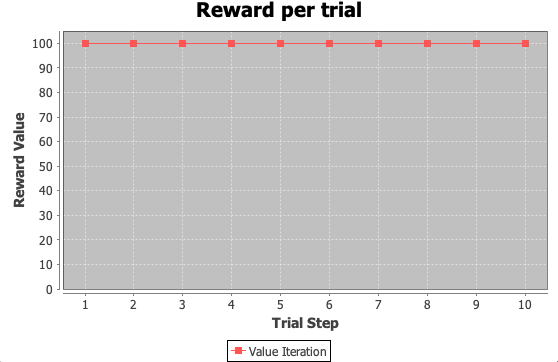
\includegraphics[width=1\linewidth]{valueiterproblem2.png}
            \caption{Value Iteration \problemtwo}\label{Fig:Value Iteration \problemtwo}
        \end{minipage}
        \begin{minipage}{0.5\textwidth}
            \centering
            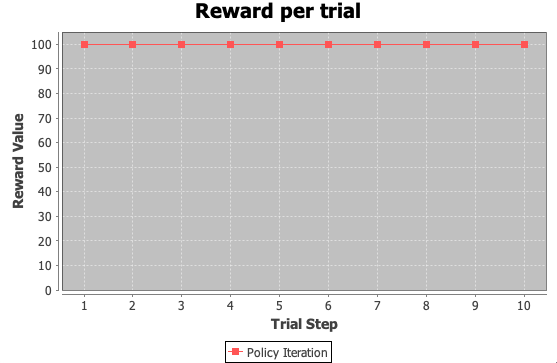
\includegraphics[width=1\linewidth]{policyiterproblem2.png}
            \caption{Policy Iteration \problemone}\label{Fig:Policy Iteration \problemtwo}
        \end{minipage}
    \end{figure}
    \begin{figure}
        \begin{minipage}{0.5\textwidth}
            \centering
            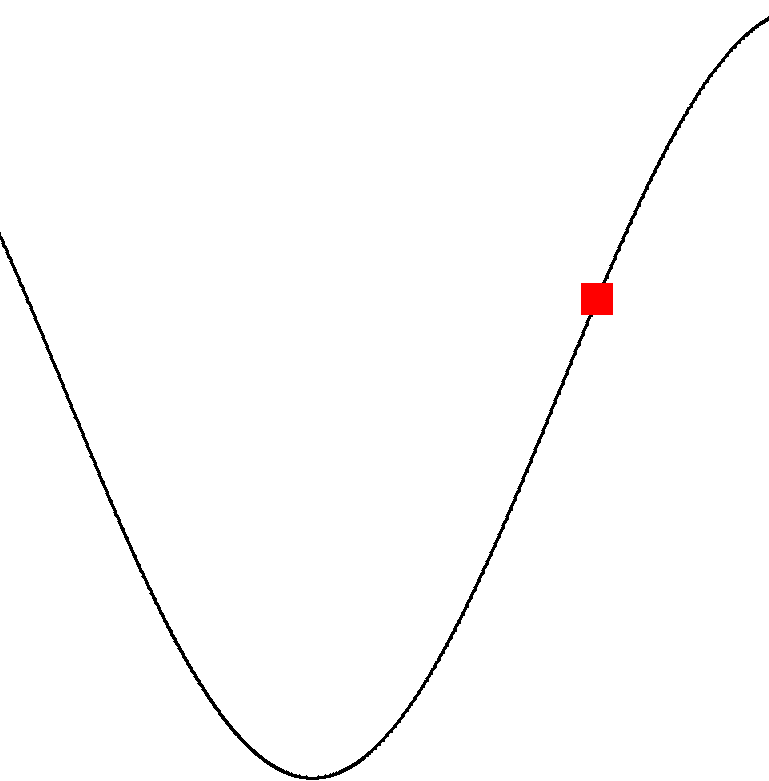
\includegraphics[width=1\linewidth]{mcgif.png}
            \caption{Mountain Car Domain}\label{Fig:Mountain Car}
        \end{minipage}
        \begin{minipage}{0.5\textwidth}
            \centering
            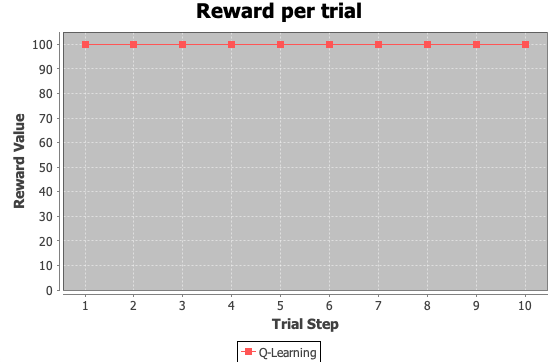
\includegraphics[width=1\linewidth]{qlearningproblem2.png}
            \caption{Q-Learning \problemtwo}\label{Fig:Q-Learning \problemtwo}
        \end{minipage}
    \end{figure}

    \begin{figure}
        \begin{minipage}{0.5\textwidth}
            \centering
            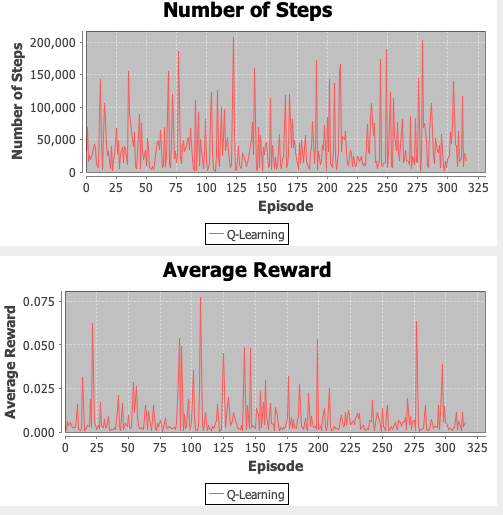
\includegraphics[width=1\linewidth]{qlearningextended.png}
            \caption{Q-Learning Deep Dive \problemtwo}\label{Fig:Q-Learning Deep Dive \problemtwo}
        \end{minipage}
    \end{figure}


    \section{Conclusion}
    In this paper I have explored the tradeoffs between several popular MDP solving algorithms in BURLAP.
    I have compared them in two different novel problems which exercised and demonstrated the differences and similarities
    in terms of performance of these algorithms.
    \bibliography{bibliography}
    \bibliographystyle{plain}
\end{document}